\documentclass[11pt,oneside]{book}
\usepackage[english, italian]{babel} 
\usepackage{microtype}
\usepackage[utf8]{inputenc}
\usepackage{subfigure}
\usepackage{epsfig}
\usepackage{amsmath, amssymb}
\usepackage[linesnumbered,lined,commentsnumbered,italiano]{algorithm2e}
\usepackage{fancybox}
\usepackage{listings}
\usepackage{url}
\usepackage{graphicx}
\usepackage{todonotes}
\usepackage{moreverb}
\usepackage{lmodern}
\usepackage{multirow}
\usepackage[labelfont=it,textfont={it}]{caption}
\usepackage[final,bookmarks,breaklinks,colorlinks,allcolors=black]{hyperref}
\usepackage{color}
\usepackage[block=ragged,backend=biber,natbib=true]{biblatex} % Use the bibtex backend with the authoryear citation style (which resembles APA)
\addbibresource{bibliography.bib} % The filename of the bibliography
\usepackage[autostyle=true]{csquotes} % Required to generate language-dependent quotes in the bibliography
\usepackage{hyperref}
\usepackage{enumitem}

%%%%%%%%%%%%%%%%%%%%%%%%%%%%
\definecolor{mygreen}{rgb}{0,0.6,0}
\definecolor{mygray}{rgb}{0.5,0.5,0.5}
\definecolor{mymauve}{rgb}{0.58,0,0.82}
\lstset{ %
	backgroundcolor=\color{white},   % choose the background color; you must add \usepackage{color} or \usepackage{xcolor}; should come as last argument
	basicstyle=\footnotesize,        % the size of the fonts that are used for the code
	breakatwhitespace=false,         % sets if automatic breaks should only happen at whitespace
	breaklines=true,                 % sets automatic line breaking
	captionpos=b,                    % sets the caption-position to bottom
	commentstyle=\color{mygreen},    % comment style
	deletekeywords={...},            % if you want to delete keywords from the given language
	escapeinside={\%*}{*)},          % if you want to add LaTeX within your code
	extendedchars=true,              % lets you use non-ASCII characters; for 8-bits encodings only, does not work with UTF-8
	frame=single,
	keepspaces=true,                 % keeps spaces in text, useful for keeping indentation of code (possibly needs columns=flexible)
	keywordstyle=\color{blue},       % keyword style
	morekeywords={*,...},            % if you want to add more keywords to the set
	numbers=left,                    % where to put the line-numbers; possible values are (none, left, right)
	numberstyle=\tiny\color{mygray}, % the style that is used for the line-numbers
	rulecolor=\color{black},         % if not set, the frame-color may be changed on line-breaks within not-black text (e.g. comments (green here))
	showspaces=false,                % show spaces everywhere adding particular underscores; it overrides 'showstringspaces'
	showstringspaces=false,          % underline spaces within strings only
	showtabs=false,                  % show tabs within strings adding particular underscores
	stringstyle=\color{mymauve},     % string literal style
	tabsize=2,	                   % sets default tabsize to 2 spaces
	title=\lstname                   % show the filename of files included with \lstinputlisting; also try caption instead of title
}
%%%%%%%%%%%%%
\definecolor{gray}{rgb}{0.4,0.4,0.4}
\definecolor{darkblue}{rgb}{0.0,0.0,0.6}
\definecolor{cyan}{rgb}{0.0,0.6,0.6}

%%%%%%%%%%%%%%%%%%%%%%%%
\begin{document}
\selectlanguage{italian}

\begin{titlepage}
\begin{center}

\epsfig{file=Figure/logo_standard.jpg,width=2.5truecm}\\[0.2truecm]
{\Large Universit\`a degli Studi di Salerno}\\[0.2truecm]
{\large Dipartimento di Informatica}\\
\hrulefill
\vfill
{\Large GameUp }\\[0.2truecm]
\vfill\vfill
{\Huge Object Design Document}
\vfill\vfill


{\bf Studenti} \hfill {\bf Docente}\ \ \\
Francesco Foglia \hfill Prof. Andrea De Lucia\\

\vfill
\hrulefill 

Anno Accademico 2020-2021

\end{center}
\end{titlepage}

\pagenumbering{roman}
\chapter*{Cronologia Revisioni}
\begin{center}
	\begin{tabular}{||c c p{10cm}||} 
	\hline
	Data & Versione & Descrizione \\ [0.5ex] 
	\hline\hline
	20/01/2021 & 0.1 & Conversione in formato TeX dell'intero documento e release iniziale \\
	\hline
	24/01/2021 & 1.0 & Completamento interfacce e class diagram completi\\
	\hline
   \end{tabular}
\end{center}

\tableofcontents
\pagestyle{plain}

%%%%%%%%%%%%%%%%%%%%%%%%%%%%
\chapter{Introduzione}
\setcounter{page}{1} 	% devono seguire solo il primo capitolo
\pagenumbering{arabic}	% devono seguire solo il primo capitolo
\input{01ODD_introduzione.tex}

%%%%%%%%%%%%%%%%%%%%%%%%%%%%
\chapter{Packages}
La divisione del sistema in packages verrà realizzata tramite una esatta gerarchia del filesystem del progetto. La struttura di base usata è quella proposta dal framework Laravel, dove in particolare:
\begin{itemize}
	\item La cartella app conterrà tutto il codice per gestire le richieste dei clienti, dall’arrivo della richiesta ad un controller fino all’invio di una risposta;
	\item La cartella database conterrà il codice relativo alla generazione della nostra fonte di dati relazionale, ovvero le migrazioni contenenti gli schemi delle nostre tabelle (così da avere una traccia dei cambiamenti applicati nel tempo al database) ed eventuali classi seeder per il riempimento di dati mock per il testing;
	\item La cartella resources conterrà tutta la parte di front end del nostro sistema, categorizzato in tre sottocartelle:
	\begin{itemize}
		\item css per i fogli di stile;
		\item js per il codice JavaScript client-side;
		\item views per i documenti rappresentanti le interfacce proposte agli utenti;
		\end{itemize}
\end{itemize}

In particolare, la cartella \emph{app} sarà quella dove verrà collocata la gran parte del nostro sistema. La sua struttura è come segue:
\begin{itemize}
	\item Exceptions, contenente le definizioni delle eccezioni lanciate dal nostro sistema;
	\item Http, contenente una cartella Controllers dove verranno realizzati i nostri Controller per ogni pagina del sistema, assieme ad una cartella \emph{Middleware} per eventuali middleware customizzati;
	\item Models, contenente i nostri modelli Eloquent per interfacciarci con il database relazionale;
\end{itemize}

Inoltre, verranno create due cartelle all’interno della cartella \emph{app} per i layer ulteriori individuati durante la fase di individuazione di design patterns:
\begin{itemize}
	\item Services, contenente i servizi offerti dal nostro sistema, raggruppati in cartelle che rappresentano i sottosistemi ai quali fanno parte;
	\item Repositories, contenente l’interfaccia Repository e le repositories per l’accesso ai dati persistenti gestiti dal sistema;
\end{itemize}

%%%%%%%%%%%%%%%%%%%%%%%%%%%%
\chapter{Interfacce delle Classi}
Le classi che comporranno il nostro back end saranno di cinque tipi: Model, Controller, Services, Repositories e le classi PHP rappresentanti gli oggetti trattati dalla logica di business. I model e gli oggetti della logica di business non avranno bisogno di una descrizione della loro interfaccia, poiché non avranno implementazioni relative alla logica di business: il loro obiettivo è di fornire un punto di accesso tramite il paradigma ad oggetti al database relazionale per i primi, mentre i secondi servono come rappresentazione orientata ad oggetti dei dati trattati dal sistema; i servizi useranno questi dati per costruire risposte da fornire ai controller. Il front end sarà composto semplicemente da dei template riempiti con i dati forniti dai controller. Il flusso di esecuzione generale sarà sempre composto da un oggetto Control che chiama un metodo di un oggetto Service per eseguire un servizio, senza mai accedere direttamente agli oggetti Repository; gli oggetti Service accederanno agli oggetti Repository necessari per ottenere i dati necessari; gli oggetti Repository comunicheranno con gli oggetti per l’accesso dei dati, come ad esempio i Model di Laravel.

\setlist[itemize]{noitemsep, topsep=0pt}
\section{Classi Control}
\subsection{UtenteControl}
\small\begin{tabular}{|| l | p{28em} ||} 
	\hline
	Nome & UtenteControl\\
	\hline
	Descrizione & Questo control riceve le richieste relative al sottosistema Utenza, invocando i servizi necessari per eseguire operazioni di autenticazione e di gestione del profilo. \\
	\hline
	Attributi & \begin{itemize}
		\item[-] utenzaService: UtenzaService
	\end{itemize}\\
	\hline
	Firme Metodi & \begin{itemize}
		\item[+] login(Request request): RedirectResponse
		\item[+] logout(): RedirectResponse
		\item[+] registrazione(): View
		\item[+] effettuaRegistrazione(Request request): RedirectResponse 
		\item[+] visualizzaProfilo(): View
		\item[+] modificaProfilo(): View
		\item[+] modificaDatiProfilo(Request request): RedirectResponse
		\item[+] getAvatar(): Response 
	\end{itemize}\\
	\hline
	Pre-condizioni & \begin{itemize}
		\item \textbf{context} UtenteControl::login(request)
		\begin{itemize}
			\item[ ] \textbf{pre:} request.has([‘username’, ‘password’]) and !utenzaService.isAuthenticated()
		\end{itemize}
	  
	    \item \textbf{context} UtenteControl::logout()
		\begin{itemize}
			\item[ ] \textbf{pre:} utenzaService.isAuthenticated()
		\end{itemize} 
	  
	    \item \textbf{context} UtenteControl::effettuaRegistrazione(request) 
		\begin{itemize}
			\item[ ] \textbf{pre:} request.has([‘username’, ‘email’, ‘password’, ‘confermaPassword’])
		\end{itemize} 
	  
	    \item \textbf{context} UtenteControl::visualizzaProfilo() 
		\begin{itemize}
			\item[ ] \textbf{pre:} utenzaService.isAuthenticated()
		\end{itemize} 
	  
	    \item \textbf{context} UtenteControl::modificaProfilo() 
		\begin{itemize}
			\item[ ] \textbf{pre:} utenzaService.isAuthenticated()
		\end{itemize} 

		\item \textbf{context} UtenteControl::modificaDatiProfilo(request) 
	\begin{itemize}
		\item[ ] \textbf{pre:} request.hasAny([‘username’, ‘email’, ‘isSviluppatore’, ‘avatar’, ‘nuovaPassword’]) and utenzaService.isAuthenticated() and request.has('passwordAttuale')
	\end{itemize}

	\item \textbf{context} UtenteControl::getAvatar() 
	\begin{itemize}
		\item[ ] \textbf{pre:} utenzaService.isAuthenticated()
	\end{itemize} 
	\end{itemize}\\
	\hline
\end{tabular}

\newpage
\paragraph{UtenteControl}
\small\begin{tabular}{|| l | p{28em} ||}
	\hline
	Post-condizioni & \begin{itemize}
		\item \textbf{context} UtenteControl::login(request)
		\begin{itemize}
			\item[ ] \textbf{post:} utenzaService.isAuthenticated()
		\end{itemize}
	  
	    \item \textbf{context} UtenteControl::logout()
		\begin{itemize}
			\item[ ] \textbf{post:} !utenzaService.isAuthenticated()
		\end{itemize} 
	  
	    \item \textbf{context} UtenteControl::registrazione(request) 
		\begin{itemize}
			\item[ ] \textbf{post:} utenzaService.isAuthenticated() and utenzaService.usernameExists(request.input(‘username’)) and utenzaService.emailExists(request.input('email'))
		\end{itemize} 

	    \item \textbf{context} UtenteControl::modificaDatiProfilo(request) 
		\begin{itemize}
			\item[ ] \textbf{post:} utenzaService.getUtenteAutenticato().username == request.input(‘username’) and utenzaService.getUtenteAutenticato().email == request.input(‘email’) and utenzaService.getUtenteAutenticato().isSviluppatore == request.input(‘isSviluppatore’) and utenzaService.getUtenteAutenticato().avatar == request.input(‘avatar’)
		\end{itemize} 
	\end{itemize}\\
	\hline
	Invarianti & \begin{itemize}
		\item \textbf{context} UtenteControl
		\begin{itemize}
			\item[ ] \textbf{inv:} utenzaService \verb|<>| null
		\end{itemize}
	\end{itemize}\\
	\hline
	\end{tabular}

\newpage
\subsection{VideogiocoControl}
\small\begin{tabular}{|| l | p{28em} ||} 
	\hline
	Nome & VideogiocoControl\\
	\hline
	Descrizione & Questo control riceve le richieste relative al sottosistema Videogioco, invocando i servizi necessari per eseguire tutte le operazioni relative ai videogiochi contenuti nel sistema. \\
	\hline
	Attributi & \begin{itemize}
		\item[-] videogiocoService: VideogiocoService
		\item[-] utenzaService: UtenzaService
	\end{itemize}\\
	\hline
	Firme Metodi & \begin{itemize}
		\item[+] ottieniDatiVideogioco(Request request): View
		\item[+] paginaIniziale(): View 
		\item[+] catalogo(Request request): View 
		\item[+] getLogo(int idVideogioco): Response
		\item[+] avviaModifica(int idVideogioco): View
		\item[+] aggiornaDatiVideogioco(Request request): RedirectResponse
		\item[+] visualizzaRichieste(): Response
		\item[+] visualizzaDettagliRichiesta(int idRichiesta): View
		\item[+] risolviRichiesta(Request request): RedirectResponse
		\item[+] richiediModificaVideogioco(): View
		\item[+] modificaDatiVideogioco(Request request): RedirectResponse
		\item[+] avviaPubblicazioneVideogioco(): View 
		\item[+] richiediPubblicazioneVideogioco(Request request): RedirectResponse
		\item[+] iniziaSponsorizzazione(): View
		\item[+] verificaDisponibilitàSettimana(Request request): JsonResponse
		\item[+] procediPagamentoSponsorizzazione(): Response
		\item[+] acquistaVideogioco(Request request): Response
		\item[+] downloadVideogioco(Request request): Response
		\item[+] avviaProceduraSuggerimentoTags(): View
		\item[+] suggerisciTags(Request request): JsonResponse
		\item[+] rimuoviSuggerimento(Request request): JsonResponse
		\item[+] salvaValutazione(Request request): JsonResponse
		\item[+] salvaRecensione(Request request): JsonResponse
	\end{itemize}\\
	\hline
\end{tabular}

\newpage
\paragraph{VideogiocoControl}
\small\begin{tabular}{|| l | p{28.5em} ||} 
\hline
Pre-condizioni & \begin{itemize}[leftmargin=*]
	\item \textbf{context} VideogiocoControl::ottieniDatiVideogioco(request)
	\begin{itemize}
		\item[ ] \textbf{pre:} request.has(‘idVideogioco’)
	\end{itemize}

	\item \textbf{context} VideogiocoControl::getLogo(idVideogioco)
	\begin{itemize}
		\item[ ] \textbf{pre:} idVideogioco \verb|<>| null
	\end{itemize}

	\item \textbf{context} VideogiocoControl::avviaModifica(idVideogioco)
	\begin{itemize}
		\item[ ] \textbf{pre:} request.has(‘idVideogioco’)
	\end{itemize}
  
	\item \textbf{context} VideogiocoControl::aggiornaDatiVideogioco(request)
	\begin{itemize}
		\item[ ] \textbf{pre:} utenzaservice.isAuthenticated() and utenzaService.isAdmin() and request.has(‘idVideogioco’) and request.hasAny([‘logo’, ‘titolo’, ‘immagini’, ‘descrizione’, ‘prezzo’]) 
	\end{itemize} 
  
	\item \textbf{context} VideogiocoControl::visualizzaRichieste()
	\begin{itemize}
		\item[ ] \textbf{pre:} utenzaService.isAdmin()
	\end{itemize} 
  
	\item \textbf{context} VideogiocoControl::visualizzaDettagliRichiesta(idRichiesta)
	\begin{itemize}
		\item[ ] \textbf{pre:} utenzaService.isAdmin() and idRichiesta \verb|<>| null
	\end{itemize} 
  
	\item \textbf{context} VideogiocoControl::risolviRichiesta(request)
	\begin{itemize}
		\item[ ] \textbf{pre:} utenzaservice.isAuthenticated() and utenzaService.isAdmin() and request.has([‘idRichiesta’, ‘esito’, ‘commento’])
	\end{itemize} 
  
	\item \textbf{context} VideogiocoControl::modificaDatiVideogioco(request)
	\begin{itemize}
		\item[ ] \textbf{pre:} utenzaService.isSviluppatore() and request.has(‘idVideogioco’) and request.hasAny([‘logo’, ‘titolo’, ‘immagini’, ‘descrizione’, ‘prezzo’]) 
	\end{itemize}

	\item \textbf{context} VideogiocoControl::avviaPubblicazioneVideogioco(request)
	\begin{itemize}
		\item[ ] \textbf{pre:} utenzaService.isSviluppatore()
	\end{itemize} 
  
	\item \textbf{context} VideogiocoControl::\newline
	richiediPubblicazioneVideogioco(request)
	\begin{itemize}
		\item[ ] \textbf{pre:} utenzaService.isSviluppatore() and request.has([‘logo’, ‘titolo’, ‘immagini’, ‘descrizione’, ‘prezzo’, ‘eseguibile’])
	\end{itemize}

	\item \textbf{context} VideogiocoControl::iniziaSponsorizzazione()
	\begin{itemize}
		\item[ ] \textbf{pre:} utenzaService.isSviluppatore()
	\end{itemize}

	\item \textbf{context} VideogiocoControl::\newline
	verificaDisponibilitàSettimana(request)
	\begin{itemize}
		\item[ ] \textbf{pre:} utenzaService.isSviluppatore() and request.has(‘settimana’) 
	\end{itemize}
	
	\item \textbf{context} VideogiocoControl::\newline
	procediPagamentoSponsorizzazione(request)
	\begin{itemize}
		\item[ ] \textbf{pre:} utenzaService.isSviluppatore() and request.has([‘idVideogioco’, ‘settimane’]) and videogiocoService.settimaneDisponibili(request.input(‘settimane’))
	\end{itemize}

	\item \textbf{context} VideogiocoControl::acquistaVideogioco(request)
	\begin{itemize}
		\item[ ] \textbf{pre:} utenzaService.isAuthenticated() and request.has(‘idVideogioco’)
	\end{itemize}
\end{itemize}\\
\hline
\end{tabular}

\newpage
\paragraph{VideogiocoControl}
\small\begin{tabular}{|| l | p{28.5em} ||} 
\hline
Pre-condizioni & \begin{itemize}[leftmargin=*]
	\item \textbf{context} VideogiocoControl::downloadVideogioco(request)
	\begin{itemize}
		\item[ ] \textbf{pre:} utenzaService.isAuthenticated()
		and request.hasAll([‘idVideogioco’, ‘versione’])
		and videogiocoService.getVideogiochiAcquistati()\verb|->| includes(videogiocoService\newline .getVideogioco(request.input(‘idVideogioco’)))	
	\end{itemize}

	\item \textbf{context} VideogiocoControl::avviaProceduraSuggerimentoTags()
	\begin{itemize}
		\item[ ] \textbf{pre:} utenzaService.isAuthenticated()
		and request.has(‘idVideogioco’)
		and videogiocoService.getVideogiochiAcquistati()\verb|->| includes(videogiocoService\newline .getVideogioco(request.input(‘idVideogioco’)))
	\end{itemize}

	\item \textbf{context} VideogiocoControl::suggerisciTags(request)
	\begin{itemize}
		\item[ ] \textbf{pre:} utenzaService.isAuthenticated() and request.hasAll([‘idVideogioco’, ‘tags’])
		and videogiocoService.getVideogiochiAcquistati()\verb|->|includes(videogiocoService\newline .getVideogioco(request.input(‘idVideogioco’)))
	\end{itemize}

	\item \textbf{context} VideogiocoControl::rimuoviSuggerimento(request)
	\begin{itemize}
		\item[ ] \textbf{pre:} utenzaService.isAuthenticated()
		and request.hasAll([‘idVideogioco’, ‘tags’])
		and videogiocoService.getTagsSuggerite(request.input(‘idVideogioco’))\verb|->|intersection(request.input(‘tags’))\verb|->|size \verb|<>| 0	
	\end{itemize}

	\item \textbf{context} VideogiocoControl::salvaValutazione(request)
	\begin{itemize}
		\item[ ] \textbf{pre:} utenzaService.isAuthenticated() and request.has(‘idRecensione’) and videogiocoService.getValutazioneRecensione(request.input(‘idRecensione’)) == null
	\end{itemize}

	\item \textbf{context} VideogiocoControl::salvaRecensione(request)
	\begin{itemize}
		\item[ ] \textbf{pre:} utenzaService.isAuthenticated() and request.has(‘idVideogioco’) and videogiocoService.getRecensione(request.input(‘idVideogioco)) == null
	\end{itemize}
\end{itemize}\\
\hline
\end{tabular}

\newpage
\paragraph{VideogiocoControl}
\small\begin{tabular}{|| l | p{28em} ||} 
\hline
Post-condizioni & \begin{itemize}[leftmargin=*]
	\item \textbf{context} VideogiocoControl::aggiornaDatiVideogioco(request)
	\begin{itemize}
		\item[ ] \textbf{post:} request.all()\verb|->|forAll(k: string, v: string $|$ videogiocoService.getVideogioco(request.input(‘id’))[k] == v)	
	\end{itemize}

	\item \textbf{context} VideogiocoControl::risolviRichiesta(request)
	\begin{itemize}
		\item[ ] \textbf{post:} videogiocoService.getRichiesta(request.input(‘idRichiesta’)).esito == request.input(‘esito’) and videogiocoService.getRichiesta(request.input(‘idRichiesta’)).commento == request.input(‘commento’)
	\end{itemize}

	\item \textbf{context} VideogiocoControl::modificaDatiVideogioco(request)
	\begin{itemize}
		\item[ ] \textbf{post:} videogiocoService.
		getVideogioco(request.input(‘idVideogioco’)
		.getRichieste()\verb|->|size ==
		videogiocoService
		.getVideogioco(request.input(‘idVideogioco’)
		@pre.getRichieste()\verb|->|size + 1	
	\end{itemize}

	\item \textbf{context} VideogiocoControl\newline ::richiediPubblicazioneVideogioco(request)
	\begin{itemize}
		\item[ ] \textbf{post:} utenzaService
		.getRichieste(utenzaService\newline .getUtenteAutenticato())\verb|->|size ==
		utenzaService
		@pre.getRichieste(utenzaService\newline .getUtenteAutenticato())\verb|->|size + 1	
	\end{itemize}

	\item \textbf{context} VideogiocoControl::suggerisciTags(request)
	\begin{itemize}
		\item[ ] \textbf{post:} videogiocoService\newline .getTags(request.input(‘idVideogioco))\newline \verb|->|intersection(request.input(‘tags’)) == request.input(‘tags’)
	\end{itemize}
\end{itemize}\\
\hline
\end{tabular}

\newpage
\paragraph{VideogiocoControl}
\small\begin{tabular}{|| l | p{28em} ||} 
\hline
Post-condizioni & \begin{itemize}[leftmargin=*]
	\item \textbf{context} VideogiocoControl::rimuoviSuggerimento(request)
	\begin{itemize}
		\item[ ] \textbf{post:} videogiocoService.getTagsSuggerite(\newline request.input(‘idVideogioco’))\verb|->|intersection(request\newline .input(‘tags’))\verb|->|size == 0
	\end{itemize}

	\item \textbf{context} VideogiocoControl::salvaRecensione(request)
	\begin{itemize}
		\item[ ] \textbf{post:} videogiocoService.getRecensione(request.input(‘idVideogioco’)) \verb|<>| null
	\end{itemize}
\end{itemize}\\
\hline
Invarianti & \begin{itemize}
	\item \textbf{context} VideogiocoControl
	\begin{itemize}
		\item[ ] \textbf{inv:} videogiocoService \verb|<>| null and utenzaService \verb|<>| null
	\end{itemize}
\end{itemize}\\
\hline
\end{tabular}

\newpage
\subsection{ForumControl}
\small\begin{tabular}{|| l | p{34em} ||} 
	\hline
	Nome & ForumControl\\
	\hline
	Descrizione & Questo control riceve le richieste relative al sottosistema Forum, invocando i servizi necessari per eseguire tutte le operazioni relative alle discussioni e ai commenti contenuti nel sistema. \\
	\hline
	Attributi & \begin{itemize}
		\item[-] videogiocoService: VideogiocoService
		\item[-] utenzaService: UtenzaService
		\item[-] forumService: ForumService
	\end{itemize}\\
	\hline
	Firme Metodi & \begin{itemize}
		\item[+] chiudiDiscussione(Request request): RedirectResponse
		\item[+] creaNuovaDiscussione(Request request): View
		\item[+] creaDiscussione(Request request): RedirectResponse
		\item[+] commenta(Request request): JsonResponse
		\item[+] poniInRilievo(Request request): JsonResponse
	\end{itemize}\\
	\hline
Pre-condizioni & \begin{itemize}[leftmargin=*]
	\item \textbf{context} ForumControl::chiudiDiscussione(request)
	\begin{itemize}
		\item[ ] \textbf{pre:} utenzaservice.isAuthenticated()
		and request.has(‘idDiscussione’)
		and forumService
		  .checkPermessiDiscussione(request.input(‘idDiscussione’))
		and forumService
		  .getDiscussione(request.input(‘idDiscussione’)).chiusa == false	
	\end{itemize}

	\item \textbf{context} ForumControl::creaNuovaDiscussione(request)
	\begin{itemize}
		\item[ ] \textbf{pre:} utenzaservice.isAuthenticated()
		and request.has(‘idVideogioco’)
		and videogiocoService.getVideogiochiAcquistati() \verb|->|includes(\newline videogiocoService.getVideogioco(request.input('idVideogioco')))
	\end{itemize}

	\item \textbf{context} ForumControl::creaDiscussione(request)
	\begin{itemize}
		\item[ ] \textbf{pre:} utenzaservice.isAuthenticated()
		and request.hasAll([‘idVideogioco’, ‘titolo’, ‘corpo’])
		and videogiocoService.getVideogiochiAcquistati() \verb|->|includes(\newline videogiocoService.getVideogioco(request.input('idVideogioco')))
	\end{itemize}

\end{itemize}\\
\hline
\end{tabular}

\newpage
\paragraph{ForumControl}
\small\begin{tabular}{|| l | p{28em} ||} 
\hline
Pre-condizioni & \begin{itemize}[leftmargin=*]
	\item \textbf{context} ForumControl::commenta(request)
	\begin{itemize}
		\item[ ] \textbf{pre:} utenzaservice.isAuthenticated()
		and request.hasAll([‘idDiscussione, ‘corpo’])
		and videogiocoService.getVideogiochiAcquistati() \verb|->|includes(\newline videogiocoService.getVideogioco(\newline request.input('idVideogioco')))	
	\end{itemize}

	\item \textbf{context} ForumControl::poniInRilievo(request)
	\begin{itemize}
		\item[ ] \textbf{pre:} utenzaservice.isAuthenticated() and request.has(‘idDiscussione’) and forumService\newline .checkPermessiDiscussione(request.input(‘idDiscussione’)) and forumService\newline .getDiscussione(request.input(‘idDiscussione’)).in\_rilievo == false
	\end{itemize}
\end{itemize}\\
\hline
Post-condizioni & \begin{itemize}[leftmargin=*]
	\item \textbf{context} ForumControl::chiudiDiscussione(request)
	\begin{itemize}
		\item[ ] \textbf{post:} forumService.getDiscussione(\newline request.input(‘idDiscussione’)).chiusa == true
	\end{itemize}

	\item \textbf{context} ForumControl::creaDiscussione(request)
	\begin{itemize}
		\item[ ] \textbf{post:} forumService.getNumDiscussioni(\newline request.input(‘idVideogioco’)) == forumService@pre.getNumDiscussioni(request.input(‘idVideogioco’)) + 1
	\end{itemize}

	\item \textbf{context} ForumControl::commenta(request)
	\begin{itemize}
		\item[ ] \textbf{post:} forumService\newline .getNumCommenti(request.input(‘idDiscussione’)) == forumService\newline @pre.getNumCommenti(request.input(‘idDiscussione’)) + 1
	\end{itemize}

	\item \textbf{context} ForumControl::poniInRilievo(request)
	\begin{itemize}
		\item[ ] \textbf{post:} forumService\newline .getDiscussione(request.input(‘idDiscussione’)).in\_rilievo == true
	\end{itemize}
\end{itemize}\\
\hline
Invarianti & \begin{itemize}
	\item \textbf{context} ForumControl
	\begin{itemize}
		\item[ ] \textbf{inv:} forumService \verb|<>| null and videogiocoService \verb|<>| null and utenzaService \verb|<>| null
	\end{itemize}
\end{itemize}\\
\hline
\end{tabular}

\newpage
\section{Classi Service}
\subsection{Utenza Service}
\small\begin{tabular}{|| l | p{34em} ||} 
	\hline
	Nome & UtenzaService\\
	\hline
	Descrizione & Questo service rende disponibili tutte le funzionalità relative all'autenticazione, all'autorizzazione e quelle relative ai singoli utenti come la gestione del proprio profilo. \\
	\hline
	Attributi & \begin{itemize}
		\item[-] utenzaRepository: UtenzaRepository
	\end{itemize}\\
	\hline
	Firme Metodi & \begin{itemize}
		\item[+] login(string username, string password): boolean
		\item[+] logout(): void
		\item[+] registraUtente(string username, string password, string email, UploadedFile avatar = null): boolean
		\item[+] getUtenteAutenticato(): ?Utenza
		\item[+] modificaDatiProfilo(string passwordAttuale, string username, string nuovaPassword, string email, boolean isSviluppatore, UploadedFile avatar)
		\item[+] usernameExists(string username): boolean
		\item[+] emailExists(string email): boolean
		\item[+] isAdmin(): boolean 
		\item[+] isSviluppatore(): boolean 
		\item[+] getAvatar(): string 
		\item[+] getRichieste(): array 
	\end{itemize}\\
	\hline
Pre-condizioni & \begin{itemize}[leftmargin=*]
	\item \textbf{context} UtenzaService::login(username, password)
	\begin{itemize}
		\item[ ] \textbf{pre:} utenzaRepository.allUsers()\verb|->| exists(u: Utente $|$ u.username == username and u.password == Hash::make(password))
	\end{itemize}

	\item \textbf{context} UtenzaService::registraUtente(username, password, email, avatar)
	\begin{itemize}
		\item[ ] \textbf{pre:} !usernameExists(username) and !emailExists(email)
	\end{itemize}

	\item \textbf{context} UtenzaService::modificaDatiProfilo(passwordAttuale, username, email, avatar, isSviluppatore)
	\begin{itemize}
		\item[ ] \textbf{pre:} utenzaRepository.checkPassword(Auth::id(), passwordAttuale) and !emailExists(email) and !usernameExists(username)
	\end{itemize}

	\item \textbf{context} UtenzaService::getRichieste()
	\begin{itemize}
		\item[ ] \textbf{pre:} isSviluppatore()
	\end{itemize}

\end{itemize}\\
\hline
\end{tabular}

\newpage
\paragraph{Utenza Service}
\small\begin{tabular}{|| l | p{28em} ||} 
\hline
Post-condizioni & \begin{itemize}[leftmargin=*]
	\item \textbf{context} UtenzaService::login(username, password)
	\begin{itemize}
		\item[ ] \textbf{post:} getUtenteAutenticato().username == username
	\end{itemize}

	\item \textbf{context} UtenzaService::logout()
	\begin{itemize}
		\item[ ] \textbf{post:} getUtenteAutenticato() == null
	\end{itemize}
	
	\item \textbf{context} UtenzaService::registraUtente(passwordAttuale, username, password, email, avatar)
	\begin{itemize}
		\item[ ] \textbf{post:} getUtenteAutenticato().username == username and getUtenteAutenticato().password == Hash::make(password) and getUtenteAutenticato().email == email and Hash::make(getUtenteAutenticato().avatar) == Hash::make(avatar)
	\end{itemize}
	
	\item \textbf{context} UtenzaService::modificaDatiProfilo(username, email, avatar, isSviluppatore)
	\begin{itemize}
		\item[ ] \textbf{post:} (username == null or getUtenteAutenticato().username == username) and (email == null or getUtenteAutenticato().email == email) and (avatar == null or Hash::make(getUtenteAutenticato().avatar) == Hash::make(avatar)) and (isSviluppatore == null or ((isSviluppatore() and isSviluppatore) or (!isSviluppatore() and !isSviluppatore))
	\end{itemize}
\end{itemize}\\
\hline
Invarianti & \begin{itemize}
	\item \textbf{context} UtenzaService
	\begin{itemize}
		\item[ ] \textbf{inv:} utenzaRepository \verb|<>| null
	\end{itemize}
\end{itemize}\\
\hline
\end{tabular}

\newpage
\subsection{Videogioco Service}
\small\begin{tabular}{|| l | p{28em} ||} 
	\hline
	Nome & VideogiocoService\\
	\hline
	Descrizione & Questo service rende disponibili tutte le funzionalità relative alla gestione dei videogiochi e oggetti correlati, come le sponsorizzazioni, le richieste e le versioni di un videogioco. \\
	\hline
	Attributi & \begin{itemize}
		\item[-] videogiocoRepository: VideogiocoRepository
		\item[-] utenzaService: UtenzaService
		\item[-] pagamentoService: PagamentoService 
	\end{itemize}\\
	\hline
	Firme Metodi & \begin{itemize}
		\item[+] ottieniDatiVideogioco(int idVideogioco): ?Videogioco
		\item[+] applicaCriteri(string titolo = null, float prezzo = null, array tagsObbligatorie = null, array tagsOpzionali = null, boolean acquistati = false, string ordine = 'DESC'): Collection
		\item[+] ottieniVideogiochiSponsorizzati(Carbon data = null): Collection
		\item[+] ottieniVideogiochiPiùScaricati(): Collection
		\item[+] ottieniUltimiVideogiochiPubblicati(): Collection
		\item[+] ottieniVideogiochiSimili(): Collection
		\item[+] aggiornaDatiVideogioco(int idVideogioco, UploadedFile logo = null, string titolo = null, array immagini = null, string descrizione = null, float prezzo = null): void
		\item[+] ottieniSintesiRichieste(): array
		\item[+] ottieniDettagliRichiesta(int idRichiesta): Richiesta
		\item[+] risolviRichiesta(int idRichiesta, boolean esito, string commento): void
		\item[+] modificaDatiVideogioco(int idVideogioco, UploadedFile logo = null, string titolo = null, array immagini = null, string descrizione = null, float prezzo = null): void
		\item[+] richiediPubblicazioneVideogioco(UploadedFile logo, string titolo, array immagini, string descrizione, float prezzo, UploadedFile eseguibile): void
		\item[+] verificaDisponibilitàSettimana(Carbon settimana): boolean
		\item[+] procediPagamentoSponsorizzazione(int idVideogioco, array settimane): void
		\item[+] acquistaVideogioco(int idVideogioco): void
		\item[+] getEseguibileVideogioco(int idVideogioco, string versione): File
		\item[+] suggerisciTags(int idVideogioco, array tags): void
	\end{itemize}\\
	\hline
\end{tabular}

\newpage
\paragraph{Videogioco Service}
\small\begin{tabular}{|| l | p{28em} ||} 
	\hline
	Firme Metodi & \begin{itemize}
		\item[+] rimuoviSuggerimento(int idVideogioco, array tags): void
		\item[+] salvaValutazione(int idRecensione, boolean giudizio): void
		\item[+] getTagsSuggerite(int idVideogioco): array
		\item[+] getValutazioneRecensione(int idRecensione): ValutazioneRecensione
		\item[+] salvaRecensione(int idVideogioco, boolean giudizio, string commento): void
		\item[+] getRecensione(int idVideogioco): Recensione
	\end{itemize}\\
	\hline
	Pre-condizioni & \begin{itemize}[leftmargin=*]
		\item \textbf{context} VideogiocoService::applicaCriteri(titolo, prezzo, tagsObbligatorie, tagsOpzionali, acquistati, ordine)
		\begin{itemize}
			\item[ ] \textbf{pre:} (titolo \verb|<>| null or prezzo \verb|<>| null or tagsObbligatorie \verb|<>| null or tagsOpzionali \verb|<>| null) and (ordine == 'DESC' or ordine == 'ASC')
		\end{itemize}

		\item \textbf{context} VideogiocoService::\newline ottieniVideogiochiSponsorizzati(data)
		\begin{itemize}
			\item[ ] \textbf{pre:} data \verb|<>| null
		\end{itemize}

		\item \textbf{context} VideogiocoService::ottieniVideogiochiSimili()
		\begin{itemize}
			\item[ ] \textbf{pre:} utenzaService.isAuthenticated()
		\end{itemize}

		\item \textbf{context} VideogiocoService::\newline aggiornaDatiVideogioco(idVideogioco, logo, titolo, immagini, descrizione, prezzo)
		\begin{itemize}
			\item[ ] \textbf{pre:} videogiocoRepository.getVideogioco(idVideogioco) \verb|<>| null and (logo \verb|<>| null or titolo \verb|<>| null or immagini \verb|<>| null or immagini\verb|->|size \verb|<>| 0 or descrizione \verb|<>| null or prezzo \verb|<>| null)
		\end{itemize}

		\item \textbf{context} VideogiocoService::\newline ottieniDettagliRichiesta(idRichiesta)
		\begin{itemize}
			\item[ ] \textbf{pre:} videogiocoRepository.getRichiesta(idRichiesta) \verb|<>| null
		\end{itemize}
	\end{itemize}\\
	\hline
\end{tabular}

\newpage
\paragraph{Videogioco Service}
\small\begin{tabular}{|| l | p{28em} ||} 
	\hline
	Pre-condizioni & \begin{itemize}[leftmargin=*]
		\item \textbf{context} VideogiocoService::risolviRichiesta(idRichiesta, esito, commento)
		\begin{itemize}
			\item[ ] \textbf{pre:} videogiocoRepository.getRichiesta(idRichiesta) \verb|<>| null and utenzaService.isAdmin() and esito \verb|<>| null
		\end{itemize}

		\item \textbf{context} VideogiocoService::\newline modificaDatiVideogioco(idVideogioco, logo, titolo, immagini, descrizione, prezzo)
		\begin{itemize}
			\item[ ] \textbf{pre:} videogiocoRepository.getVideogioco(idVideogioco) \verb|<>| null and (logo \verb|<>| null or titolo \verb|<>| null or immagini \verb|<>| null or immagini\verb|->|size \verb|>| 0 or descrizione \verb|<>| null or prezzo \verb|<>| null)
		\end{itemize}

		\item \textbf{context} VideogiocoService::\newline richiediPubblicazioneVideogioco(logo, titolo, immagini, descrizione, prezzo, eseguibile)
		\begin{itemize}
			\item[ ] \textbf{pre:} utenzaService.isSviluppatore()
		\end{itemize}

		\item \textbf{context} VideogiocoService::\newline procediPagamentoSponsorizzazione(idVideogioco, settimane)
		\begin{itemize}
			\item[ ] \textbf{pre:}videogiocoRepository.getVideogioco(idVideogioco) \verb|<>| null and settimane\verb|->|size \verb|<>| 0 
		\end{itemize}

		\item \textbf{context} VideogiocoService::acquistaVideogioco(idVideogioco)
		\begin{itemize}
			\item[ ] \textbf{pre:} videogiocoRepository.getVideogioco(idVideogioco) \verb|<>| null
		\end{itemize}

		\item \textbf{context} VideogiocoService::\newline getEseguibileVideogioco(idVideogioco, versione)
		\begin{itemize}
			\item[ ] \textbf{pre:} videogiocoRepository.getVideogioco(idVideogioco) \verb|<>| null and videogiocoRepository\newline .getVersioniVideogioco(idVideogioco)\verb|->|includes(versione)
		\end{itemize}

		\item \textbf{context} VideogiocoService::suggerisciTags(idVideogioco, tags)
		\begin{itemize}
			\item[ ] \textbf{pre:} utenzaService.isAuthenticated() and videogiocoRepository.getVideogioco(idVideogioco) \verb|<>| null and videogiocoRepository\newline .getCompratori(idVideogioco)\verb|->|includes(\newline utenzaService.getUtenteAutenticato()) and tags\verb|->|size \verb|<>| 0
		\end{itemize}
	\end{itemize}\\
	\hline
\end{tabular}

\newpage
\paragraph{Videogioco Service}
\small\begin{tabular}{|| l | p{28em} ||} 
	\hline
	Pre-condizioni & \begin{itemize}[leftmargin=*]
		\item \textbf{context} VideogiocoService::rimuoviSuggerimenti(idVideogioco, tags)
		\begin{itemize} \item[ ] \textbf{pre:} utenzaService.isAuthenticated() and videogiocoRepository.getVideogioco(idVideogioco) \verb|<>| null and videogiocoRepository\newline .getCompratori(idVideogioco)\verb|->|includes(\newline utenzaService.getUtenteAutenticato()) and tags \verb|<>| null and tags\verb|->|size \verb|<>| 0
		\end{itemize}

		\item \textbf{context} VideogiocoService::salvaValutazione(idRecensione, giudizio)
		\begin{itemize}
			\item[ ] \textbf{pre:} utenzaService.isAuthenticated() and videogiocoRepository.getVideogioco(idVideogioco) \verb|<>| null and videogiocoRepository\newline .getCompratori(idVideogioco)\verb|->|includes(\newline utenzaService.getUtenteAutenticato()) and tags \verb|<>| null and tags\verb|->|size \verb|<>| 0 and giudizio \verb|<>| null
		\end{itemize}

		\item \textbf{context} VideogiocoService::getTagsSuggerite(idVideogioco)
		\begin{itemize}
			\item[ ] \textbf{pre:} utenzaService.isAuthenticated() and videogiocoRepository.getVideogioco(idVideogioco) \verb|<>| null
		\end{itemize}

		\item \textbf{context} VideogiocoService::\newline getValutazioneRecensione(idRecensione)
		\begin{itemize}
			\item[ ] \textbf{pre:} utenzaService.isAuthenticated() and videogiocoRepository.getRecensione(idRecensione) \verb|<>| null
		\end{itemize}

		\item \textbf{context} VideogiocoService::salvaRecensione(idVideogioco, giudizio, commento)
		\begin{itemize}
			\item[ ] \textbf{pre:} utenzaService.isAuthenticated() and videogiocoRepository.getVideogioco(idVideogioco) \verb|<>| null
		\end{itemize}

		\item \textbf{context} VideogiocoService::getRecensione(idVideogioco)
		\begin{itemize}
			\item[ ] \textbf{pre:} utenzaService.isAuthenticated() and videogiocoRepository.getVideogioco(idVideogioco) \verb|<>| null
		\end{itemize}
	\end{itemize}\\
	\hline
\end{tabular}

\newpage
\paragraph{Videogioco Service}
\small\begin{tabular}{|| l | p{28em} ||} 
	\hline
	Post-condizioni & \begin{itemize}[leftmargin=*]
		\item \textbf{context} VideogiocoService::ottieniVideogiochiPiùScaricati()
		\begin{itemize}
			\item[ ] \textbf{post:} result\verb|->|sortedBy(videogioco $|$ -videogioco.acquisti\verb|->|size)
		\end{itemize}

		\item \textbf{context} VideogiocoService\newline ::ottieniUltimiVideogiochiPubblicati()
		\begin{itemize}
			\item[ ] \textbf{post:} result\verb|->|sortedBy(videogioco $|$ -videogioco.created\_at.timestamp)
		\end{itemize}

		\item \textbf{context} VideogiocoService::ottieniSintesiRichieste()
		\begin{itemize}
			\item[ ] \textbf{post:} result->forAll(richiesta $|$ richiesta.titolo \verb|<>| null and richiesta.descrizione \verb|<>| null and richiesta.tipo \verb|<>| null)
		\end{itemize}

		\item \textbf{context} VideogiocoService::risolviRichiesta(idRichiesta, esito, commento)
		\begin{itemize}
			\item[ ] \textbf{post:} videogiocoRepository.getRichiesta(idRichiesta).esito == esito and videogiocoRepository.getRichiesta(idRichiesta).commento == commento
		\end{itemize}

		\item \textbf{context} VideogiocoService\newline ::verificaDisponibilitàSettimana(settimana)
		\begin{itemize}
			\item[ ] \textbf{post:} videogiocoRepository.getSponsorizzazioni\newline\verb|->|forAll(sponsorizzazione $|$ sponsorizzazione.data\_inizio.startOfWeek() \verb|<>| settimana.startOfWeek() and sponsorizzazione.data\_fine.endOfWeek() \verb|<>| settimana.endOfWeek()) and result == true
		\end{itemize}

		\item \textbf{context} VideogiocoService::suggerisciTags(idVideogioco, tags)
		\begin{itemize}
			\item[ ] \textbf{post:} videogiocoRepository\newline .getTagsVideogioco(idVideogioco)\verb|->|intersection(tags) == tags
		\end{itemize}

		\item \textbf{context} VideogiocoService::rimuoviSuggerimenti(idVideogioco, tags)
		\begin{itemize}
			\item[ ] \textbf{post:} videogiocoRepository\newline .getTagsVideogioco(idVideogioco)\verb|->|intersection(tags)\newline \verb|->|size == 0
		\end{itemize}
	\end{itemize}\\
	\hline
	Invarianti & \begin{itemize}
		\item \textbf{context} VideogiocoService
		\begin{itemize}
			\item[ ] \textbf{inv:} videogiocoRepository \verb|<>| null and utenzaService \verb|<>| null and pagamentoService \verb|<>| null
		\end{itemize}
	\end{itemize}\\
	\hline
\end{tabular}

\subsection{Forum Service}
\small\begin{tabular}{|| l | p{28em} ||} 
	\hline
	Nome & ForumService\\
	\hline
	Descrizione & Questo service rende disponibili tutte le funzionalità relative alla gestione dei forum relativi ai singoli videogiochi, con le relative discussioni e commenti associati. \\
	\hline
	Attributi & \begin{itemize}
		\item[-] forumRepository: ForumRepository
		\item[-] videogiocoService: VideogiocoService
		\item[-] utenzaService: UtenzaService
	\end{itemize}\\
	\hline
	Firme Metodi & \begin{itemize}
		\item[+] chiudiDiscussione(int idDiscussione): void
		\item[+] creaDiscussione(int videogiocoId, string titolo, string corpo): Discussione
		\item[+] commenta(int idDiscussione, string corpo): Commento
		\item[+] poniInRilievo(int idDiscussione): void
	\end{itemize}\\
	\hline
	Pre-condizioni & \begin{itemize}[leftmargin=*]
		\item \textbf{context} ForumService::chiudiDiscussione(idDiscussione)
		\begin{itemize}
			\item[ ] \textbf{pre:} utenzaService.isAuthenticated() and forumRepository.getDiscussione(idDiscussione) \verb|<>| null and videogiocoService\newline .ottieniDatiVideogioco(forumRepository\newline .getDiscussione(idDiscussione).idVideogioco).autore == utenzaService.getUtenteAutenticato()
		\end{itemize}

		\item \textbf{context} ForumService::creaDiscussione(idVideogioco, titolo, corpo)
		\begin{itemize}
			\item[ ] \textbf{pre:} videogiocoService\newline .ottieniDatiVideogioco(idVideogioco) \verb|<>| null and videogiocoRepository\newline .getCompratori(idVideogioco)\verb|->|includes(\newline utenzaService.getUtenteAutenticato())
		\end{itemize}

		\item \textbf{context} ForumService::commenta(idDiscussione, corpo)
		\begin{itemize}
			\item[ ] \textbf{pre:} forumRepository.getDiscussione(idDiscussione) \verb|<>| null and videogiocoRepository\newline .getCompratori(forumRepository\newline .getDiscussione(idDiscussione).idVideogioco)\verb|->|includes(\newline utenzaService.getUtenteAutenticato())
		\end{itemize}

		\item \textbf{context} ForumService::poniInRilievo(idDiscussione)
		\begin{itemize}
			\item[ ] \textbf{pre:} forumRepository.getDiscussione(idDiscussione) \verb|<>| null and forumRepository.getDiscussione(idDiscussione).in\_rilievo == false
		\end{itemize}
	\end{itemize}\\
	\hline
\end{tabular}

\paragraph{Forum Service}
\small\begin{tabular}{|| l | p{28em} ||} 
	\hline
	Post-condizioni & \begin{itemize}[leftmargin=*]
		\item \textbf{context} ForumService::chiudiDiscussione(idDiscussione)
		\begin{itemize}
			\item[ ] \textbf{post:} forumRepository.\newline getDiscussione(idDiscussione).chiusa == true
		\end{itemize}

		\item \textbf{context} ForumService::commenta(idDiscussione, corpo)
		\begin{itemize}
			\item[ ] \textbf{post:} forumRepository.getCommenti(idDiscussione)\verb|->|size == forumRepository\newline @pre.getCommenti(idDiscussione)\verb|->|size + 1
		\end{itemize}

		\item \textbf{context} ForumService::poniInRilievo(idDiscussione)
		\begin{itemize}
			\item[ ] \textbf{post:} forumRepository\newline .getDiscussione(idDiscussione).in\_rilievo == true
		\end{itemize}
	\end{itemize}\\
	\hline
	Invarianti & \begin{itemize}
		\item \textbf{context} ForumService
		\begin{itemize}
			\item[ ] \textbf{inv:} forumRepository \verb|<>| null and  videogiocoService \verb|<>| null and utenzaService \verb|<>| null
		\end{itemize}
	\end{itemize}\\
	\hline
\end{tabular}

\newpage
\subsection{Pagamento Service}
\small\begin{tabular}{|| l | p{28em} ||} 
	\hline
	Nome & PagamentoService\\
	\hline
	Descrizione & Questo service gestisce i pagamenti relativi all'acquisto di videogiochi e di sponsorizzazioni, esponendo un metodo ciascuno per astrarre la comunicazione con il provider esterno del servizio di pagamento online. \\
	\hline
	Attributi & \begin{itemize}
		\item[-] videogiocoService: VideogiocoService
	\end{itemize}\\
	\hline
	Firme Metodi & \begin{itemize}
		\item[+] avviaPagamento(int idVideogioco): void 
		\item[+] procediPagamento(int idVideogioco): void
		\item[+] callbackStripeAcquisto(int idUtente, int idVideogioco): void  
		\item[+] callbackStripeSponsorizzazione(int idUtente, int idVideogioco): void
	\end{itemize}\\
	\hline
	Pre-condizioni & \begin{itemize}[leftmargin=*]
		\item \textbf{context} PagamentoService::avviaPagamento(idVideogioco)
		\begin{itemize}
			\item[ ] \textbf{pre:} videogiocoService.getVideogioco(idVideogioco) \verb|<>| null
		\end{itemize}

		\item \textbf{context} PagamentoService::procediPagamento(idVideogioco)
		\begin{itemize}
			\item[ ] \textbf{pre:} videogiocoService.getVideogioco(idVideogioco) \verb|<>| null
		\end{itemize}
	\end{itemize}\\
	\hline
	Post-condizioni & \begin{itemize}[leftmargin=*]
		\item \textbf{context} PagamentoService::callbackStripeAcquisto(idUtente, idVideogioco)
		\begin{itemize}
			\item[ ] \textbf{post:} videogiocoService\newline .getVideogiochiAcquistati(idUtente)\verb|->|size == videogiocoService\newline @pre.getVideogiochiAcquistati(idUtente)\verb|->|size + 1
		\end{itemize}

		\item \textbf{context} PagamentoService::\newline callbackStripeSponsorizzazione(idVideogioco)
		\begin{itemize}
			\item[ ] \textbf{post:} videogiocoService\newline .getSponsorizzazioni(idVideogioco)\verb|->|size == videogiocoService\newline @pre.getSponsorizzazioni(idVideogioco)\verb|->|size + 1
		\end{itemize}
	\end{itemize}\\
	\hline
	Invarianti & \begin{itemize}
		\item \textbf{context} PagamentoService
		\begin{itemize}
			\item[ ] \textbf{inv:} videogiocoService \verb|<>| null
		\end{itemize}
	\end{itemize}\\
	\hline
\end{tabular}


\newpage
\section{Classi Repository}
\subsection{Utenza Repository}
\small\begin{tabular}{|| l | p{34em} ||} 
	\hline
	Nome & UtenzaRepository\\
	\hline
	Descrizione & Questa repository rappresenta il punto di accesso principale per la classe Utente, come astrazione dei modelli Eloquent forniti dal framework Laravel. In particolare, questa classe non ritorna mai l'hash della password degli utenti agli strati superiori.\\
	\hline
	Attributi & \begin{itemize}
		\item[-] N/A
	\end{itemize}\\
	\hline
	Firme Metodi & \begin{itemize}
		\item[+] allUsers(): array
		\item[+] getUtente(int idUtente): ?Utenza
		\item[+] findUsername(string username): ?Utenza
		\item[+] findEmail(string email): ?Utenza
		\item[+] createUtente(string username, string password, string email, UploadedFile avatar = null): Authenticatable
		\item[+] modificaDatiProfilo(int idUtente, string username = null, string nuovaPassword = null, string email = null, boolean isSviluppatore = null, UploadedFile avatar = null): boolean
		\item[+] checkPassword(int idUtente, string password): boolean    
	\end{itemize}\\
	\hline
Pre-condizioni & \begin{itemize}[leftmargin=*]
	\item \textbf{context} UtenzaRepository::modificaDatiProfilo(idUtente, username, password, email, isSviluppatore, avatar)
	\begin{itemize}
		\item[ ] \textbf{pre:} User::find(idUtente) \verb|<>| null
	\end{itemize}
\end{itemize}\\
\hline
Post-condizioni & \begin{itemize}[leftmargin=*]
	\item \textbf{context} UtenzaRepository::getUtente(idUtente)
	\begin{itemize}
		\item[ ] \textbf{post:} result.id == idUtente
	\end{itemize}

	\item \textbf{context} UtenzaRepository::findUsername(username)
	\begin{itemize}
		\item[ ] \textbf{post:} (result == null) or (result.username == username
	\end{itemize}

	\item \textbf{context} UtenzaRepository::findEmail(email)
	\begin{itemize}
		\item[ ] \textbf{post:} (result == null) or (result.email == email
	\end{itemize}
\end{itemize}\\
\hline
Invarianti & \begin{itemize}
	\item N/A
\end{itemize}\\
\hline
\end{tabular}

\newpage
\subsection{Videogioco Repository}
\small\begin{tabular}{|| l | p{34em} ||} 
	\hline
	Nome & VideogiocoRepository\\
	\hline
	Descrizione & Questa repository rappresenta il punto di accesso principale per la classe Videogioco e le classi strettamente correlate, ovvero Tags, Versioni, Sponsorizzazioni, Recensioni e ValutazioneRecensioni, assieme alle classi pivot di collegamento che collegano una di queste con altre classi, astraendo la comunicazione con i modelli di Eloquent per i dati relazionali e con il filesystem per i file.\\
	\hline
	Attributi & \begin{itemize}
		\item[-] N/A
	\end{itemize}\\
	\hline
	Firme Metodi & \begin{itemize}
		\item[+] getVideogioco(int idVideogioco): ?Videogioco
		\item[+] applicaCriteri(string titolo = null, float prezzo = null, array tagsObbligatorie = null, array tagsOpzionali = null, int idUtente = null, boolean acquistati = false, string ordine = 'DESC'): array
		\item[+] creaVideogioco(Videogioco videogioco): void 
		\item[+] aggiornaDatiVideogioco(Videogioco videogioco): void
		\item[+] getVersioniVideogioco(int idVideogioco): array 
		\item[+] getRichiesta(int idRichiesta): Richiesta  
	\end{itemize}\\
	\hline
Pre-condizioni & \begin{itemize}[leftmargin=*]
	\item \textbf{context} VideogiocoRepository::getVersioniVideogioco(idVideogioco)
	\begin{itemize}
		\item[ ] \textbf{pre:} Videogiochi::find(idVideogioco) \verb|<>| null
	\end{itemize}
\end{itemize}\\
\hline
Post-condizioni & \begin{itemize}[leftmargin=*]
	\item N/A
\end{itemize}\\
\hline
Invarianti & \begin{itemize}
	\item N/A
\end{itemize}\\
\hline
\end{tabular}

\newpage
\subsection{Forum Repository}
\small\begin{tabular}{|| l | p{34em} ||} 
	\hline
	Nome & ForumRepository\\
	\hline
	Descrizione & Questa repository rappresenta il punto di accesso principale per le classi Discussioni e Commenti.\\
	\hline
	Attributi & \begin{itemize}
		\item[-] N/A
	\end{itemize}\\
	\hline
	Firme Metodi & \begin{itemize}
		\item[+] getDiscussione(int idDiscussione): ?Discussione
		\item[+] getCommenti(int idDiscussione): array 
		\item[+] creaCommento(int idDiscussione, string corpo): void
		\item[+] creaDiscussione(string titolo, string corpo): void
	\end{itemize}\\
	\hline
Pre-condizioni & \begin{itemize}[leftmargin=*]
	\item \textbf{context} ForumRepository::getCommenti(idDiscussione)
	\begin{itemize}
		\item[ ] \textbf{pre:} getDiscussione(idDiscussione) \verb|<>| null
	\end{itemize}

	\item \textbf{context} ForumRepository::creaCommento(idDiscussione)
	\begin{itemize}
		\item[ ] \textbf{pre:} getDiscussione(idDiscussione) \verb|<>| null
	\end{itemize}
\end{itemize}\\
\hline
Post-condizioni & \begin{itemize}[leftmargin=*]
	\item N/A
\end{itemize}\\
\hline
Invarianti & \begin{itemize}
	\item N/A
\end{itemize}\\
\hline
\end{tabular}

\subsection{Class Diagrams}
\subsubsection{Sistema Utenza}
\begin{center}
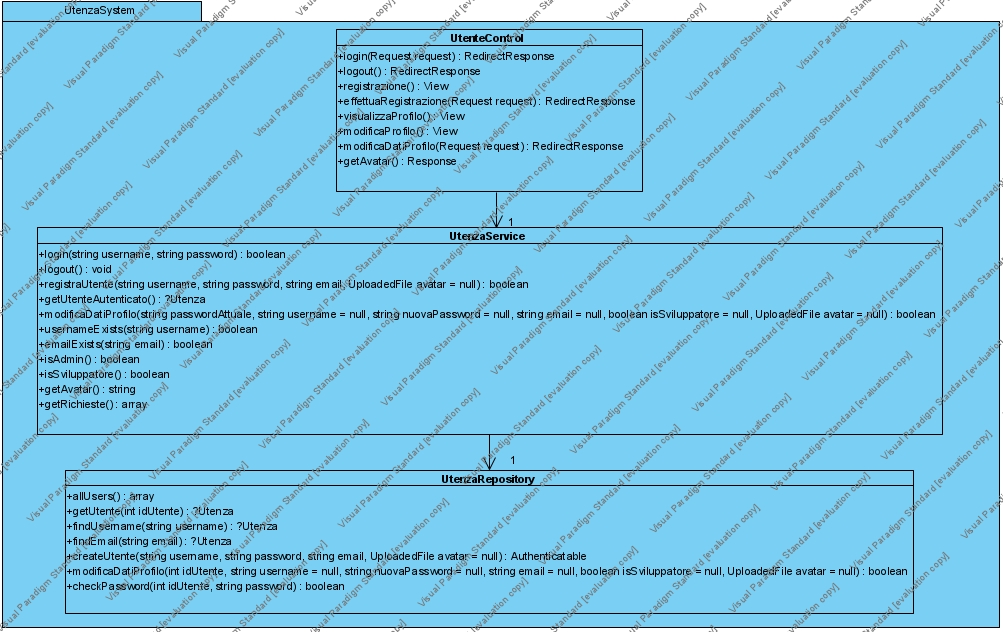
\includegraphics[width=\textwidth,height=\textheight,keepaspectratio]{Figure/ClassDiagramUtenza.jpg}
\end{center}

\subsubsection{Sistema Videogiochi}
\begin{center}
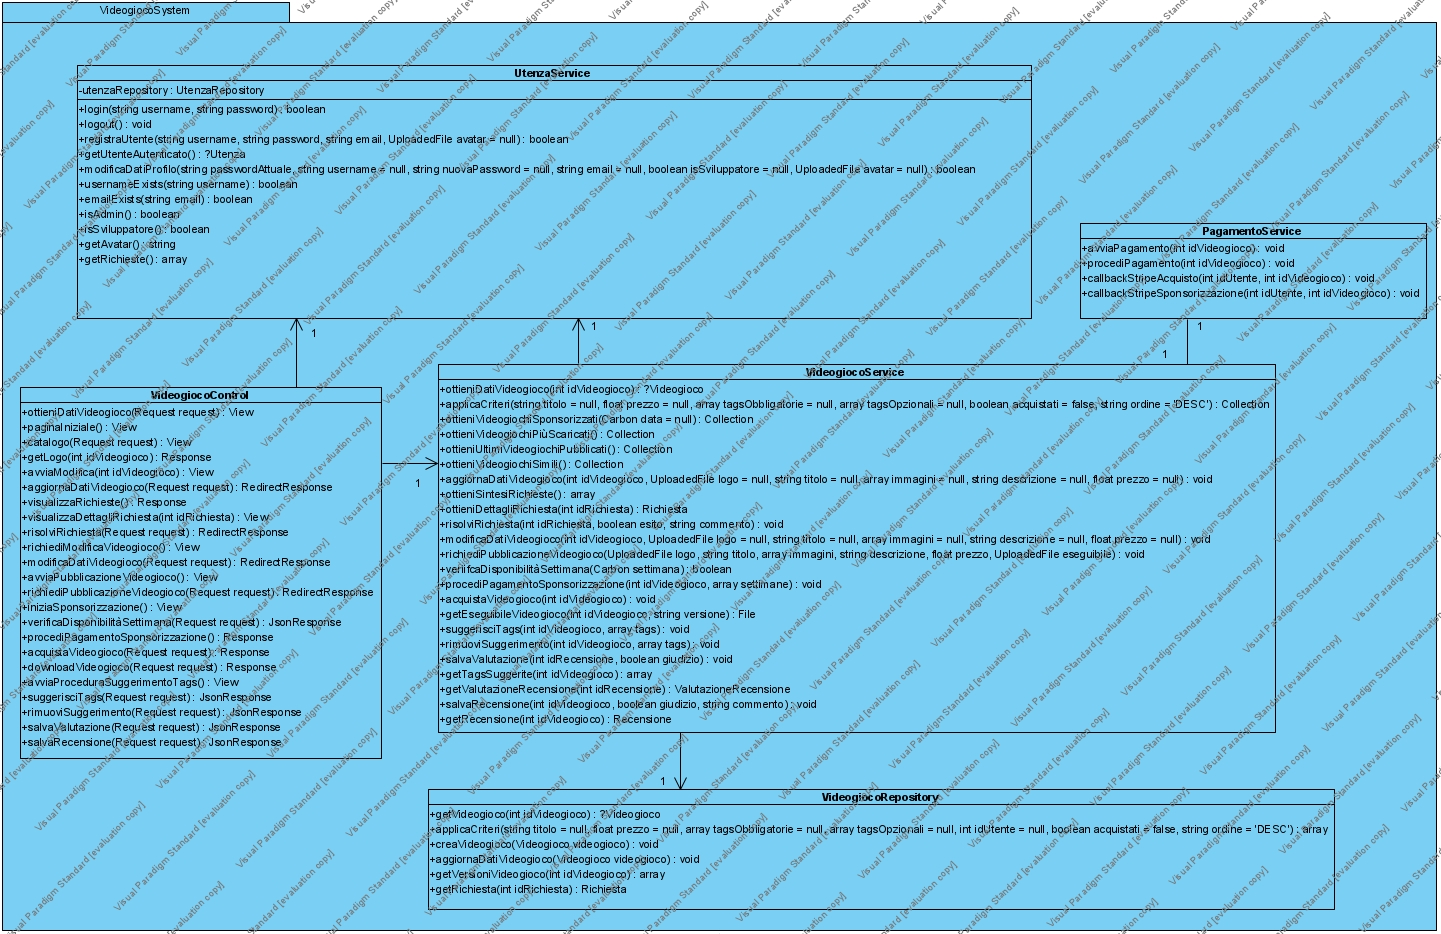
\includegraphics[width=\textwidth,height=\textheight,keepaspectratio]{Figure/ClassDiagramVideogioco.jpg}
\end{center}

\subsubsection{Sistema Forum}
\begin{center}
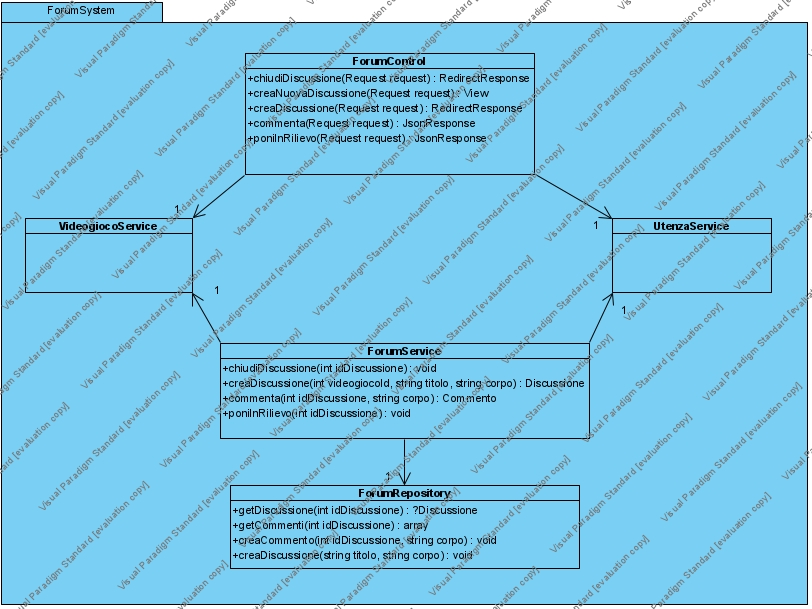
\includegraphics[width=\textwidth,height=\textheight,keepaspectratio]{Figure/ClassDiagramForum.jpg}
\end{center}


%%%%%%%%%%%%%%%%%%%%%%%%%%%%
\end{document}
